\documentclass[11pt]{article} 

\usepackage{deauthor,times,graphicx}
%\usepackage{url}
\usepackage{hyperref}


\begin{document}
%\title{Data Caching Systems Win the Cost/Performance Game}

%\author{David Lomet\\Microsoft Research\\Redmond, WA 98052\\lomet@microsoft.com}
 

%\maketitle

\section{Introduction}

\subsection{Cost/Performance}

Data in traditional data caching record management systems resides on secondary storage, and is read into main memory only when operated on.  This limits system performance.  Main memory data stores with data always in main memory are faster.  But this performance comes at an increased cost.  The analysis in \cite{Damon} shows how modern data caching systems can produce better cost/performance.  Their exploition of a storage hierarchy hence can serve a greater diversity of data management needs at lower cost.


\subsection{A Little History}

Traditional data management systems were implemented using hard disk drives (HDD) coupled with small main memories.  Such systems were, of necessity, designed as data caching systems.  That is, data lived on HDDs, and was read into a main memory cache to be operated on.  As main memories became larger and costs fell, more and more data was cached.  Removing I/O cost from the path to data improved performance substantially.  It exposed, however, new performance bottlenecks.  For example, concurrency control and recovery (CCR) has modest execution cost compared with data I/O accesses.  With the I/O cost reduced, CCR became a much larger part of operation execution path. 

Database researchers, in striving for great performance, looked again at CCR.  Ultimately, high performance CCR techniques were developed that depended, for effectiveness, upon there being no I/O. High latency within transactions did not fit well with these techniques. This led to main memory only data management systems, e.g., \cite{diaconu, hyper13,voltdb}, with performance of millions of operations/sec. Main memory systems inspired an explosion of new CCR and data access techniques suitable for such systems.  However, the performance gains required permanently committing main memory to the data being managed. 

The main memory efforts have, however, led to technology that made it possible to achieve much higher performance in data caching systems.  For example, both  RocksDB~\cite{rocksdb} and Deuteronomy~\cite{LLS13,LLS13a,TC} use main memory techniques, e.g. latch-free data access, for high performance on data cached in main memory.   In addition, both dramatically shrink write I/O cost via log structuring techniques, and avoid some read I/O by supporting  ``blind" updates without the pages needing to be in main memory.  

\section{Data Management Economics}

\label{sec:analysis}

A data management system should $ALWAYS$ be able to achieve higher performance with all data in main memory.  Further, the fall-off in performance when data has to first be brought into the cache is substantial, even for a highly optimized system. So why bother with a data caching system?  The answer is ``better cost/performance''.  So the argument here is not that there is insufficient main memory to hold the data, but that there is a less costly way to manage data.


We regard data caching system operations as coming in two flavors, in-memory operations $MM$ (data is in main memory) and secondary storage operations $SS$ (data needs to be brought into main memory).  Data management operations have both execution and storage costs.  Storage costs are always paid, while execution costs are incurred only when data is operated on.  $MM$ operations have higher performance (no secondary storage data access) while $SS$ operations have lower storage costs (flash is cheaper than DRAM).  


\subsection{Data Management Cost/Sec}

We analyze cost per second of data management for our two operations: $MM$ and $SS$ \footnote{A more detailed analysis is in \cite{Damon}.}  The costs are of two forms, storage rental costs for data and cpu and device rental costs for operation execution.  

{\bf $MM$ operations:} We need to rent a page of DRAM (\$DRAM) and a page of flash (\$FLASH) because the data is also on secondary storage.  $MM$ operation execution cost is \$MOP.

\begin{equation}\$MM = (\$DRAM + \$FLASH) + N*\$MOP \end{equation} 

{\bf $SS$ operations:} We need to rent a page of flash (\$FLASH) but not a page of DRAM since we are bringing the data into DRAM only as needed.  So the cost in DRAM is insignificantly small.  The cost of an $SS$ operation involves its storage cost, now flash memory, with cost \$FLASH and its execution cost \$SOP.  \$SOP consists of $MM$ operation execution cost \$MOP plus the cost of bringing the data into DRAM.  This second cost is \$FLOP, the cost of an SSD's IO operation, plus \$IO, the cost of the cpu executing its IO path .

  
\begin{equation}\$SS = \$FLASH + N*(\$MOP + \$FLOP + \$IO) \end{equation} 

We can now calculate the breakeven point- i.e., how many op/sec $N$ we need to execute for the costs to be equal.  For lowest cost, we switch between $MM$ and $SS$ operations at that point. 
We solve for $1/N$, the interval between accesses when costs are equal.
%\footnotesize
\begin{equation} \label{eq:Ti}
T_i = \frac{1}{N} = \frac{\$SOP - \$MOP}{\$DRAM} = \frac{\$FLOP + \$IO}{\$DRAM}
\end{equation}

$T_i$ yields our version of the ``5-minute" rule.  $T_i$ is approximately one minute (the updated ``5 minute rule"~\cite{gray1}). The smaller the breakeven time, the sooner the cost is reduced by evicting the page.  A data caching system can use the breakeven point in choosing the lower cost operation.   It approximates this point with its caching policy.  The cost trade-off between $MM$ and $SS$ operations is shown in Figure~\ref{fig:MMSS}. Capturing operation costs permits us to compare costs at performance points away from breakeven. This demonstrates why flash cost \$FLASH is so important.


\begin{figure}
\centering
%\includegraphics[width=.6\textwidth]{figures/SS-MMbreakeven1.png}
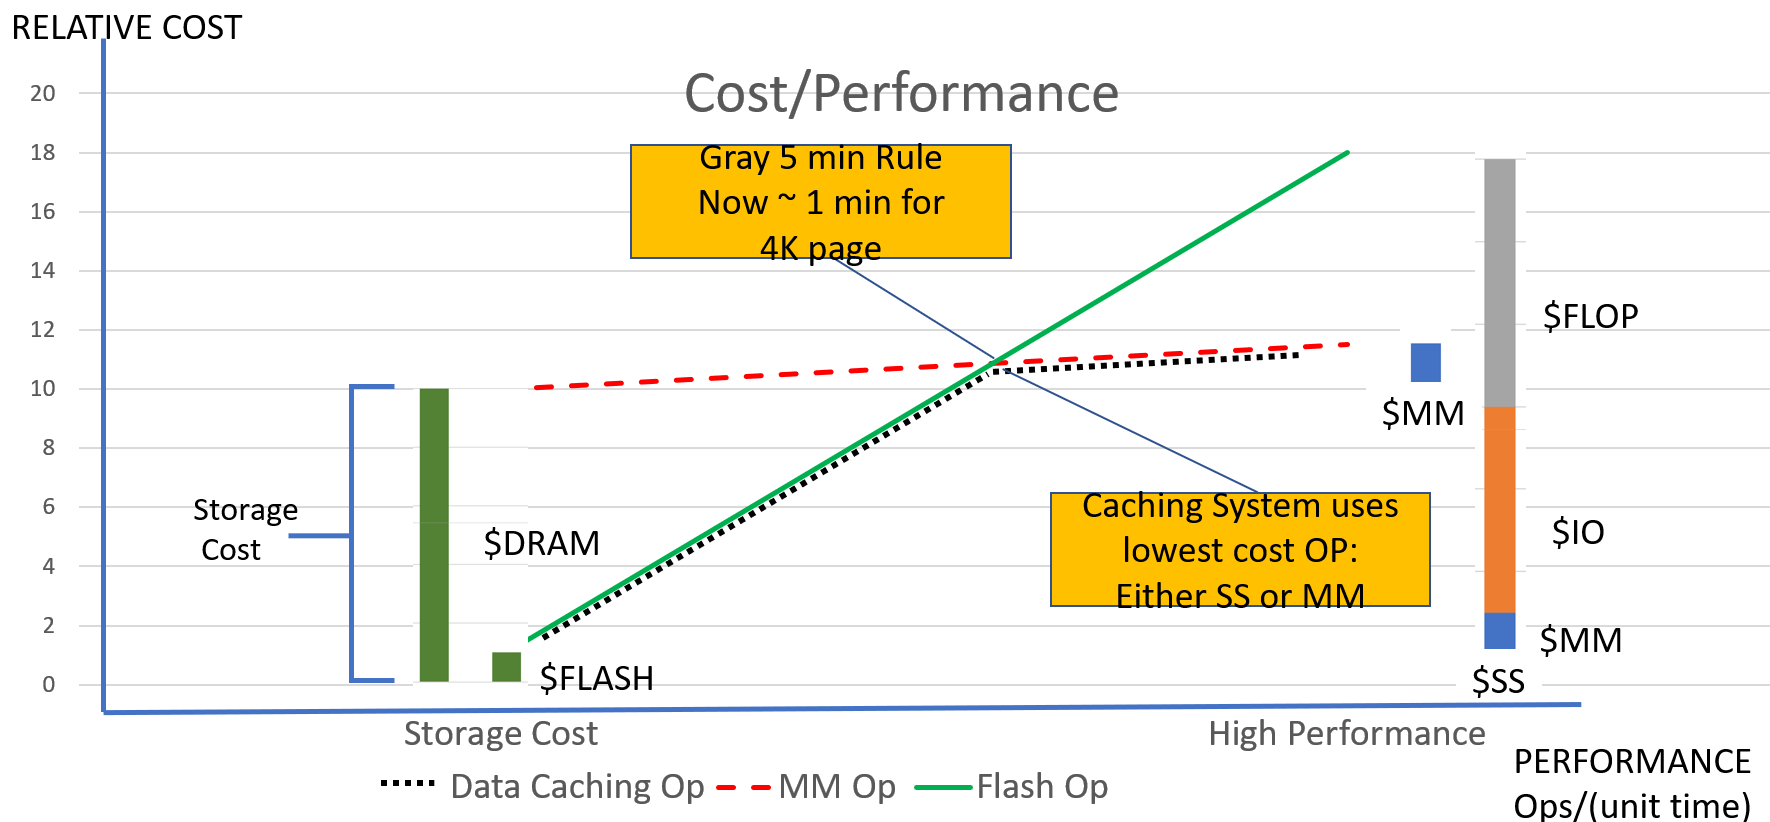
\includegraphics[height=1.7in]{letters/breakeven.png}
\caption{The cost/sec of main memory operations and secondary storage operations as execution rates change.}
\label{fig:MMSS}
\end{figure}


At low access rates, the cost of storage dominates the execution cost.  Since main memory is $10X$ more costly than flash, an $MM$ operation is $11X$ more expensive than an $SS$ operation at very low access rates.  At high access rates, it is the execution cost that dominates.  \$SOP is about $12X$ the cost of \$MOP, with \$FLOP approximately $6X$ of \$MOP, and \$IO about $5X$ of \$MOP.  The number of IOPS provide by an SSD has dramatically increased, reducing \$FLOP. Thus CPU cost (\$IO) for an I/O is now a significant part of \$SOP cost. 


Trading space (cost) for time (cost) can be useful for improving systems, but how much space for how much performance?  We analysed other technologies in~\cite{Damon} which showed similar cross-over points frequently exist where relative cost advantage also changes between systems.  Using more main memory, as done by the main memory MassTree key-value store results in its performance being higher than Deuteronomy's.  In our experiments, the breakeven point for a page at about $T_i = 3$ seconds.  Hence MassTree is better for very hot data, but not for data accessed less frequently.  Data compression saves storage cost at the expense of increasing execution cost, hence good for very cold data, even though decompression adds to execution cost.  

\vspace{-.1cm}
\section{Concluding Thoughts}

Cost/performance is usually more important than sheer performance.  And storage costs are a very big part of overall costs, since most data is cold.  Further, the hot data set typically changes over time.  Cost effective data management means reducing storage costs for cold data and reducing execution cost for hot data.  That is what data caching systems do. Data caching systems dominate the market via better cost/performance, despite main memory systems having higher performance.  

There is another message here.  Research may dramatically increase data caching system performance.  For example, reducing the cost of moving data between storage hierarchy levels could be a huge win, enabling new and cheaper storage technologies to play an important role in data management.  That research agenda might succeed in producing a "one size" system that fits (almost) all~\cite{onesizefitsall} of the data management market.



\vspace{-.1cm}
\section{Acknowledgements}
I want to thank Haixun Wang for inviting me to write this opinion piece.  Thanks also to my Deuteronomy colleagues, particularly Justin Levandoski, Sudipta Sengupta, and Ryan Stutsman.  Together, we built a great data caching system.

%\newpage
\vspace{-.1cm}
\bibliographystyle{ACM-Reference-Format}
\begin{thebibliography}{10}
\begin{small}



\itemsep=-.5pt


\bibitem{diaconu}
C. Diaconu, C. Freedman, E. Ismert, P. Larson, P. Mittal, R. Stonecipher, N. Verma, M. Zwilling:
Hekaton: SQL server's memory-optimized OLTP engine. SIGMOD 2013: 1243-1254



\bibitem{gray1}
J. Gray, G. R. Putzolu:
The 5 Minute Rule for Trading Memory for Disk Accesses and The 10 Byte Rule for Trading Memory for CPU Time. SIGMOD 1987: 395-398


\bibitem{hyper13}
A. Kemper, T. Neumann, J. Finis, F. Funke, V. Leis, H. M\"{u}lhe, T. M\"{u}hhlbauer, W. R\"{o}diger:
Processing in the Hybrid OLTP \& OLAP Main-Memory Database System HyPer. IEEE Data Eng. Bull. 36(2): 41-47 (2013)


\bibitem{LLS13}
J. Levandoski, D. Lomet, and S. Sengupta,
The Bw-Tree: A B-tree for New Hardware Platforms,
ICDE 2013, pp. 302--313.

\bibitem{LLS13a}
J. Levandoski, D. Lomet, S. Sengupta.
LLAMA: A Cache/Storage Subsystem for Modern Hardware.
PVLDB 6(10): 877-888 (2013).

\bibitem{TC}
J. Levandoski, D. Lomet, S. Sengupta, R. Stutsman, R. Wang:
High Performance Transactions in Deuteronomy.
CIDR 2015.

\bibitem{Damon}
D. Lomet: Cost/performance in modern data stores: how data caching systems succeed. DaMoN 2018: 9:1-9:10

\bibitem{rocksdb}
RocksDB: A persistent key-value store for fast storage environments.
\url{http://rocksdb.org/}

\bibitem{onesizefitsall}
M. Stonebraker, U. Cetintemel, ``One size fits all": an idea whose time has come and gone. ICDE 2005.


\bibitem{voltdb}
M. Stonebraker, A. Weisberg:
The VoltDB Main Memory DBMS. IEEE Data Eng. Bull. 36(2): 21-27 (2013)



\end{small}
\end{thebibliography}


\end{document}
